\chapter{Background}
\label{chapter:background}

\section{Alzheimer's disease}
\label{sec:AD}

%neurodegenerative diseases
Neurodegenerative diseases such as Alzheimer's disease (AD) result in progressive degeneration and death of neuron cells and affect more than 35 million people worldwide \cite{querfurth2010mechanisms}. Other neurodegenerative diseases include Parkinson's disease, Huntington's disease, Amyotrophic lateral sclerosis and Lewy bodies dementia. However, Alzheimer's disease is by far the most common type of dementia, accounting for 60\% to 70\% of the total cases of dementia \cite{Burns2009,world2013dementia}.

% AD, symptoms, age as risk
Alzheimer's disease is a progressive neurodegenerative disease that usually affects people over 65 years of age \cite{Burns2009,world2013dementia}. Its early symptoms include short-term memory loss, but as the disease advances other symptoms appear such as problems with language, disorientation, mood swings, loss of motivation and behavioural issues \cite{Burns2009,world2013dementia}. The average life expectancy after clinical diagnosis is between three to nine years, although the speed of progression can vary \cite{querfurth2010mechanisms}. The principal risk factor of AD is age, with incidence rates doubling every 5 years after 65 years of age \cite{querfurth2010mechanisms,todd2013survival}. 

% causes
Its causes are poorly understood and around 70\% of the risk is thought to be genetic, with many risk genes involved such as APOE, GSK3$\beta$, DYRK1A and many others \cite{Ballard2011alzheimers}. Other risk factors include head injuries, depression and hypertension \cite{Burns2009}. Pathologically, Alzheimer's disease is characterised by the presence of amyloid plaques and neurofibrillary tangles in the brain tissue \cite{braak1991neuropathological}. In 1991, Hardy et al. postulated that amyloid-$\beta$ deposits are a central cause in the development of AD, followed by tau phosphorylation and tangle formation and neuronal death \cite{hardy1991amyloid}. This was supported by the discovery of a pathogenic mutation in the amyloid precursor protein (APP) gene on chromosome 21 and by the occurrence of AD in Down syndrome. On the other hand, the tau hypothesis suggests that abnormalities related to the tau proteins initiate the disease cascade \cite{mudher2002alzheimer}. In this case, tau binding to microtubules is disrupted by phosphorylation which results in free tau that aggregates into neurofibrillary tangles. This ends up destroying the cell's cytoskeleton which collapses the neuron's transport system, ultimately resulting in neuronal death. 

% treatment
There are no effective treatments available to stop or reverse neuronal degeneration in AD \cite{Burns2009}. Nevertheless, there exists some medication that can temporarily reduce some symptoms or slow down the progression in some people. Among these, most of them are acetylcholinesterase inhibitors: tacrine, rivastigmine, galantamine and donepezil \cite{grossberg2003management}. Psychosocial interventions are used to complement pharmaceutical treatment, but they don't usually focus on AD but on dementia in general.

% imaging modalities
Over the last decades, various biomarkers have been developed that monitor the extent of neuronal atrophy of the brain in vivo: CSF amyloid-$\beta_{1-42}$ \cite{blennow2003csf} and amyloid PET imaging using the Pittsburgh compound B \cite{klunk2004imaging} measure amyloid plaque deposits; CSF total tau and phosphorylated tau \cite{blennow2003csf} measure neurofibrillary tangles and neuroaxonal damage; fluorodeoxyglucose (FDG) PET \cite{herholz2012use} measures metabolic activity in the brain; MRI cortical volumes, thickness and atrophy rate measured using the Boundary Shift Integral \cite{freeborough1997boundary} detect shrinkage of individual brain areas that is caused by neurodegeneration. Lastly, cognitive test scores such as the Mini-Mental State Examination (MMSE) \cite{mckhann1984clinical} are used to assess memory and cognitive performance. Characterising the trajectories of these biomarkers can help us better understand the dynamics of the disease, explain its causes and perform better differential diagnosis.


% %TODO write more on AD
% \subsection{Tau pathology}
% %TODO write more on AD
% \subsection{Neurodegeneration}
% %TODO write more on AD

\subsection{Progression of AD}
%TODO write more on AD

% disease progression in AD
Several studies have been done so far on Alzheimer's disease progression \cite{jack2010hypothetical, ridha2006tracking,fox1999correlation, scahill2002mapping, braak1991neuropathological,schott2003assessing}. It is currently believed that in AD amyloid-beta and tau proteins become abnormal first, long before symptoms occur, followed by cognitive decline such as memory loss and brain structural atrophy \cite{jack2010hypothetical,jack2013tracking}.  Neuropathological staging of AD brains showed that the earliest change in brain structure are in the medial temporal lobe, particularly in the entorhinal cortex and hippocampus \cite{braak1991neuropathological}. Afterwards, in medium stages amyloid deposits are found in almost all isocortical areas apart from primary sensory areas and motor field \cite{braak1991neuropathological}. In late stages, atrophy gets worse and spreads even further to other areas including the sensory and motor fields \cite{braak1991neuropathological}. As a result of early hippocampal and entorhinal atrophy, many volumetric MRI studies focus on these regions and show that even in mild AD the entorhinal area and hippocampus shrink by 20-25\% compared to controls \cite{jack1997medial,lehericy1994amygdalohippocampal,juottonen1999comparative,bobinski1999histological}. Results by Schott et al. \cite{schott2003assessing} and Ridha et al. \cite{ridha2006tracking} show that atrophy of the medial temporal lobe precedes the clinical onset of AD by approximately 3.5 years \cite{schott2003assessing}. 

% \subsubsection{Braak staging}
% %TODO


\section{Posterior Cortical Atrophy}
\label{sec:pca}

% general, symptoms
Posterior cortical atrophy (PCA) is an early-onset subtype of Alzheimer's disease that affects the posterior past of the brain, resulting in disruption of the visual cortex. The syndrome was first reported by Benson et al. \cite{benson1988posterior} in 1988 to describe five patients with fairly homogeneous but otherwise unclassified symptoms.  The most common symptoms include inability to read, blurred vision, light sensitivity, trouble navigating through space and issues with depth perception \cite{crutch2012posterior,borruat2013posterior}. Additional symptoms also include apraxia (disorder of movement planning), visual agnosia (object recognition deficit) and agraphia (loss of writing ability) \cite{benson1988posterior,goethals2001posterior}. These symptoms get worse as the disease progresses, with patients becoming unable to recognise familiar people and objects and difficulty navigating familiar places. Some studies \cite{andrade2010visual,andrade2012visuospatial,andrade2013visuospatial} reported visual hemineglect (difficulty seeing one half of the visual field) to be frequent in PCA patients, especially if asymmetrical atrophy takes place in the occipital areas. 

% diagnosis, neuroimaging
PCA patients face difficulties in diagnosis due to the young age at onset and the fact that there are no fully accepted diagnostic criteria. Patients are sometimes misdiagnosed with depression, anxiety or even malingering in early stages of the disease \cite{crutch2012posterior}. They are often initially referred to opticians and ophthalmologists in the belief that ocular abnormalities are causing their visual deficits, often leading to unnecessary medical procedures such as cataract surgery. Neuroimaging modalities such as magnetic resonance imaging (MRI), positron emission tomography (PET) or single photon emission computed tomography (SPECT) can aid diagnosis of PCA \cite{goldstein2011posterior}. 

% causes
The causes of PCA are still unknown, due to the rarity of the disease, gradual onset of symptoms and no fully accepted diagnostic criteria \cite{borruat2013posterior,crutch2012posterior}. The progressive neurodegeneration that characterises PCA is often attributed to Alzheimer's disease, but alternative causes including dementia with Lewy bodies, corticobasal degeneration and prion disease have also been identified \cite{crutch2012posterior}. Genetic factors that underlie PCA are also not well understood \cite{crutch2012posterior,borruat2013posterior}. Empirical findings suggest that there are no significant differences in the number of patients with a positive family history of PCA and typical AD \cite{crutch2012posterior}. Some studies also report no differences in alipoprotein E (APOE) genotypes between PCA and typical AD \cite{mendez2002posterior, tang2004clinical,rosenbloom2011distinct}. 

% treatment
There is no known efficient treatment of PCA that will reverse or stop neurodegeneration \cite{borruat2013posterior}. Patients with PCA are usually treated with the same medication as for AD, namely cholinesterase inhibitors: tacrine, rivastigmine, galantamine and donepezil \cite{borruat2013posterior}. However, there are no studies analysing the efficiency of these drugs in PCA patients \cite{borruat2013posterior}. A few non-pharmacological therapies have also been attempted recently in some patients that included psycho-educative programs \cite{videaud2012impact} or a combination of speech therapy, occupational therapy and physiotherapy \cite{weill2012physical}.

% progression
As opposed to AD, PCA has a distinct progression pattern. Studies by Hof et al. \cite{hof1997atypical} and Tang-Wei et al. \cite{tang2004clinical} show a greater concentration of senile plaques and neurofibrillary tangles in the occipital and parietal lobes and at the occipito-temporal junction. In later stages of the disease neurodegeneration spreads to anterior areas of the brain, and as a result symptoms similar to Alzheimer's disease may occur, such as memory loss.

\section{Disease Progression Models}
\label{sec:disease_prog_models}

% what is a disease progression model?
A disease progression model describes the evolution of a neurodegenerative disease, which is characterised by a set of pathological changes and symptoms that occur in the brain. Although the underlying molecular mechanisms that cause these changes are not fully understood, biomarker measurements can be used to track the state of the patient and of various anatomical structures. A disease progression model therefore characterises the temporal trajectory of these biomarkers as they go from a normal to an abnormal state. Most models will be able to provide information on the ordering of the biomarkers as they become abnormal and the biomarker rate of decline. 

% Hypothetical model of disease progression by Jack
A hypothetical model of disease progression has been proposed by Jack et al. \cite{jack2010hypothetical,jack2013tracking}, which describes the trajectory of several key biomarkers during the progression of Alzheimer's disease (fig. \ref{fig:biomk_cascade}). The model suggests that amyloid-$\beta$ and tau protein biomarkers become abnormal long before the onset of any dementia symptoms. Afterwards, during the mild cognitive impairment (MCI) phase,  cognitive functions such as memory become abnormal along with brain structure measured using MRI. These biomarkers continue to be affected in the dementia stage, while A$\beta$ and tau seem to reach a plateau at this point. This hypothesised model of disease progression is shaping the current field of AD research \cite{donohue2014estimating}.

% simple models that regress group patients in clinical symptomatic stages or regress against one variable (years from onset)
Some of the simplest disease progression model are based on symptomatic staging of patients into a small number of groups, e.g. "pre-symptomatic", "mild", "moderate" and "severe" \cite{fonteijn2012event}. They then describe the differences in biomarker measurements among these groups. Scahill et al. \cite{scahill2002mapping} devised such a method that finds changes in brain structure using voxel-based analysis of serial nonlinear-registered MRI images. Other models based on symptomatic staging are those of Dickerson et al., 2009 \cite{dickerson2009cortical} and Thomson et al. 2001 \cite{thompson2001cortical}, 2003 \cite{thompson2003dynamics}. One key limitation of these methods is that the clinical assessment is usually subjective and biased, which limits the temporal resolution of the disease progression models. This limitation is one of the main factors motivating the development of data-driven models described below. Another method by Bateman et al. \cite{bateman2012clinical} uses estimated years from onset to conduct cross-sectional analyses of baseline data in order to determine the relative order and magnitude of pathophysiological changes. However, this method can only be applied to dominantly inherited AD, due to the need to estimate the years from onset using data from parents.

% Disease progression - EBM
A range of data-driven models of disease progression have also been proposed, which do not need prior knowledge of the disease stages of subjects. One such model is the \emph{event-based model}  \cite{fonteijn2012event}, which describes disease progression as a sequence of discrete events, where each event corresponds to a biomarker becoming abnormal. The model finds the optimal ordering in which biomarkers become abnormal given the data. It has so far been used to model neurodegeneration in familial AD \cite{fonteijn2012event}, Huntington's disease \cite{fonteijn2012event} and sporadic AD \cite{young2014data}. Other discrete event models include those based on Hidden Markov Models \cite{jackson2003multistate, guihenneuc2000modeling}. The advantage of the EBM is the computational simplicity of the formulation. However, it is unable to model the time between events or the rate of biomarker decline, which limits its utility for prognosis. 

% Differential equation models
Another class of disease progression models are the \emph{differential equation models} \cite{villemagne2013amyloid,oxtoby2014learning,ashford2001modeling,yang2010quantifying,sabuncu2011dynamics,jack2013brain}. These can be used to reconstruct an average biomarker trajectory which is continuous in contrast with the discrete event-based model trajectories. The models use follow-up biomarker measurements to provide sample gradients of the biomarker trajectory and integrate a differential equation to determine the average trajectory for the entire cohort. These models have been used in a variety of settings: finding the time it takes for amyloid accumulation to become abnormal in amyloid-PET images \cite{jack2013brain}, calculate the rates of amyloid $\beta$ deposition, cerebral atrophy and cognitive decline \cite{villemagne2013amyloid}. Moreover, \emph{stochastic differential equation models} can also express the deviation from the average trajectory and have been used to analyse MRI brain volumes \cite{oxtoby2014learning}. The advantage of these models is that they can compute the rate of biomarker decline, which is very useful for prognosis at an individual level. On the other hand, there is no guarantee of correspondence across disease stage and prognosis estimates between different biomarkers \cite{Young2015data}. 

% Continuous traj models: dononue, jedynak, TODO: add schiratti
\emph{Self-modelling regression} approaches can also estimate biomarker trajectories by fitting sets of curves under the assumption of a common shape throughout the population \cite{donohue2014estimating}. These approaches have been used to determine the dynamics of regional brain volumes, cognitive tests, PET-based biomarkers and CSF amyloid-beta and tau values \cite{donohue2014estimating}. Jedynak et al. \cite{jedynak2012computational} used similar biomarkers to derive a \emph{disease progression score} and applied it to the Alzheimer's Disease Neuroimaging Initiative (ADNI) dataset. The main advantage of these models is that they provide a complete picture of the disease which is useful for clinical understanding \cite{Young2015data}. Disadvantages include risk of overfitting due to the large number of parameters that need to be estimated.

\begin{figure}
 \centering
 \includegraphics[scale=0.7]{../code/toyEBMs/biomkProg.pdf}
 \caption[Biomarker cascade by Jack et al. \cite{jack2010hypothetical}]{Dynamic biomarkers of the AD cascade as hypothesised by Jack et al. \cite{jack2010hypothetical}. A$\beta$ and tau are thought to become abnormal before the onset of any dementia symptoms, while brain structure, memory and clinical function are thought to become abnormal later, during MCI and dementia stages. Reprinted from \cite{jack2010hypothetical}.}
 \label{fig:biomk_cascade}
\end{figure}


\section{The Event-Based Model}
\label{sec:ebm}

\begin{figure}
  \centering
  \includegraphics[scale = 0.7]{../code/toyEBMs/biomkProgWithSnapshots.pdf}
  \caption[Informative and uninformative snapshots in biomarker progression]{Two hypothetical biomarker progressions along with three different snapshots, that may come from the same subject or from different subjects. The left-most and the right-most snapshots have measurements that are both either low or high, so this does not give any information regarding which biomarker becomes abnormal first. However, the middle snapshot is informative because the measurement for biomarker 1 is high while the measurement for biomarker 2 is low, which suggests that biomarker 1 becomes abnormal first.}
\end{figure}

\begin{figure}
\centering
  \begin{tikzpicture}[scale=0.97, every node/.style={scale=0.98}]
    \node[inner sep=0pt] (progWithPoints) at (-5,0) {\includegraphics[scale=0.43]{../code/toyEBMs/biomkProgWithPoints.pdf}};
    \node[inner sep=0pt] (mixModel) at (3,0) {\includegraphics[scale=0.4]{../code/toyEBMs/mixModelHist.pdf}};
    \draw[loosely dotted,line width=0.60mm, red] (2.0,0) -- (-1.8,0.8);
    \draw[loosely dotted,line width=0.60mm, blue] (3.4,1.5) -- (-1.6,-1.5);
  \end{tikzpicture}
  \caption[Event-based model - biomarker data diagram]{The left figure shows biomarker measurements for controls and patients along with the underlying hypothetical (true) progression curve. The right figure shows the mixture model for the two groups of subjects. Note that there is overlap between the biomarker values. The Gaussian fit for the control groups represents $p(x|\neg E)$, while the fit for the patients group represents $p(x|E)$.}
\end{figure}

 
The event-based model was introduced by Fonteijn et al. \cite{fonteijn2012event} in 2012 and describes the disease as a sequence of discrete events. Each event represents a change in the patient state, such as the onset of a new symptom (e.g. 'patient shows a drop in cognitive performance') or measurement of tissue pathology (e.g. 'lumbar puncture shows reduced amyloid beta'). The aim of the model is to find the ordering in which events occur given a dataset of biomarker measurements. In section \ref{sec:ebm_theory} we present the theory behind the EBM, in section \ref{sec:model_est} we present the MCMC and greedy ascent methods that are used to estimate the abnormality sequence, in section \ref{sec:mix_models} we show how to fit the mixture model parameters and in section \ref{sec:staging} we show how to stage the subjects using the EBM. 

\subsection{Theory}
\label{sec:ebm_theory}

The event-based model consists of a series of events $E_1, E_2, \dots , E_N$ and an ordering $S = [s(1), \dots, s(N)]$ which is a permutation of the integers $1,\dots, N$ creating the event ordering $E_{s(1)}, E_{s(2)},\dots, E_{s(N)}$. The set of events is specified a-priori.  Moreover, the model uses a dataset $X$ which contains a set of $X_j$ measurements for each subject $j$. Each set $X_j = \{x_{1j}, x_{2j}, \dots, x_{Nj}\}$ where $x_{ij}$ represents the value of biomarker $i$ in subject $j$ and is informative of event $E_i$ in subject $j$. 

The event-based model makes two key assumptions: first, measurements decrease monotonically as the disease progresses and second, the event ordering is the same across all patients. The first assumption fits with the hypothetical model presented by Jack et al. \cite{jack2010hypothetical} in fig. \ref{fig:biomk_cascade}. Therefore, a patient for whom event $E_i$ has occurred cannot revert to a state where event $E_i$ did not occur. This assumption is essential because it ensures snapshots are informative about the event ordering \cite{fonteijn2012event}. The second assumption is necessary to be able to aggregate information about the event ordering from the entire set of subjects. 

The aim of the event-based model is to find the probability density function  $p(S|X)$ of an event ordering given the biomarker data. One starts by fitting a model for the likelihood function $p(x_{ij}|E_i)$ the likelihood of measuring $x_{ij}$ given event $E_i$ occurred. A similar fit is obtained for $p(x_{ij}|\neg E_i)$, the likelihood of measuring $x_{ij}$ given event $E_i$ has not occurred. More information about mixture model fitting can be found in section \ref{sec:mix_models}. If a subject $j$ is at stage $k$ in the disease progression, events $E_{s(1)},\dots, E_{s(k)}$ have occurred while events $E_{s(k+1)},\dots, E_{s(N)}$ have not occurred. We can therefore define the likelihood of the data from subject $j$ given ordering $S$ as:

\begin{equation}
\label{eq:ebm1}
 p(X_j | S, k) = \prod_{i=1}^k p\left(x_{s(i),j} | E_{s(i)} \right) \prod_{i=k+1}^N p\left(x_{s(i),j} | \neg E_{s(i)}\right)
\end{equation}
 
where measurements $x_{ij}$ are assumed to be independent. Since the subject could potentially be at any stage $k$ in the progression, we integrate over $k$:

\begin{equation}
\label{eq:ebm2}
  p(X_j | S) = \sum_{k=0}^N p(k)p(X_j|S,k) 
\end{equation}

where $p(k)$ is the prior probability of the subject being at position $k$ in the sequence. A uniform prior is usually assumed here. Further assuming independence of measurements across patients we get:


\begin{equation}
\label{eq:ebm3}
 p(X|S) = \prod_{j=1}^J p(X_j | S)
\end{equation}

Combining equations \ref{eq:ebm1},\ref{eq:ebm2}, \ref{eq:ebm3} we get the total likelihood:

\begin{equation}
\label{eq:ebm4}
 p(X|S) = \prod_{j=1}^J \left[ \sum_{k=0}^N p(k) \left( \prod_{i=1}^k p\left(x_{s(i),j} | E_{s(i)} \right) \prod_{i=k+1}^N p\left(x_{s(i),j} | \neg E_{s(i)}\right) \right) \right]
\end{equation}



\newcommand{\nodeRad}{0.4cm}

\begin{figure}
\centering
\begin{tikzpicture}[scale = 0.8]
  \tikzstyle{every node}=[font=\small]

  \node (samples) at (-2.5,4) {\textbf{MCMC samples}};
  \draw (-5,3) circle [radius=\nodeRad] node (E2) {E2};
  \draw (-3.5,3) circle [radius=\nodeRad] node (E1) {E1};  
  \draw (-2,3) circle [radius=\nodeRad] node (E4) {E4};
  \draw (-0.5,3) circle [radius=\nodeRad] node (E3) {E3};
  
  \draw (-5,2) circle [radius=\nodeRad] node (E1m) {E1};
  \draw (-3.5,2) circle [radius=\nodeRad] node (E2m) {E2};  
  \draw (-2,2) circle [radius=\nodeRad] node (E4m) {E4};
  \draw (-0.5,2) circle [radius=\nodeRad] node (E3m) {E3};
  
  \draw (-5,0) circle [radius=\nodeRad] node (E2s) {E2};
  \draw (-3.5,0) circle [radius=\nodeRad] node (E1s) {E1};  
  \draw (-2,0) circle [radius=\nodeRad] node (E3s) {E3};
  \draw (-0.5,0) circle [radius=\nodeRad] node (E4s) {E4};
  
  \node (1) at (-5.7,3) {1};
  \node (2) at (-5.7,2) {2};
  \node (T) at (-5.7,0) {T};
  
  \draw[loosely dotted, line width=0.3mm] (2) -- (T);
  
  
  \draw[->,line width=0.3mm] (E2) -- (E1);
  \draw[->,line width=0.3mm] (E1) -- (E4);
  \draw[->,line width=0.3mm] (E4) -- (E3);
  
  \draw[->,line width=0.3mm] (E1m) -- (E2m);
  \draw[->,line width=0.3mm] (E2m) -- (E4m);
  \draw[->,line width=0.3mm] (E4m) -- (E3m);
  
  \draw[->,line width=0.3mm] (E2s) -- (E1s);
  \draw[->,line width=0.3mm] (E1s) -- (E3s);
  \draw[->,line width=0.3mm] (E3s) -- (E4s);
  
  % characteristic ordering 
  
  \node (ordering) at (-2.5,-2) {\textbf{Maximum Likelihood Ordering}};
  \draw (-5,-3) circle [radius=\nodeRad] node (E2c) {E2};
  \draw (-3.5,-3) circle [radius=\nodeRad] node (E1c) {E1};  
  \draw (-2,-3) circle [radius=\nodeRad] node (E4c) {E4};
  \draw (-0.5,-3) circle [radius=\nodeRad] node (E3c) {E3};

  
  \draw[->,line width=0.3mm] (E2c) -- (E1c);
  \draw[->,line width=0.3mm] (E1c) -- (E4c);
  \draw[->,line width=0.3mm] (E4c) -- (E3c);
  
  \node (pic) at (5,0) {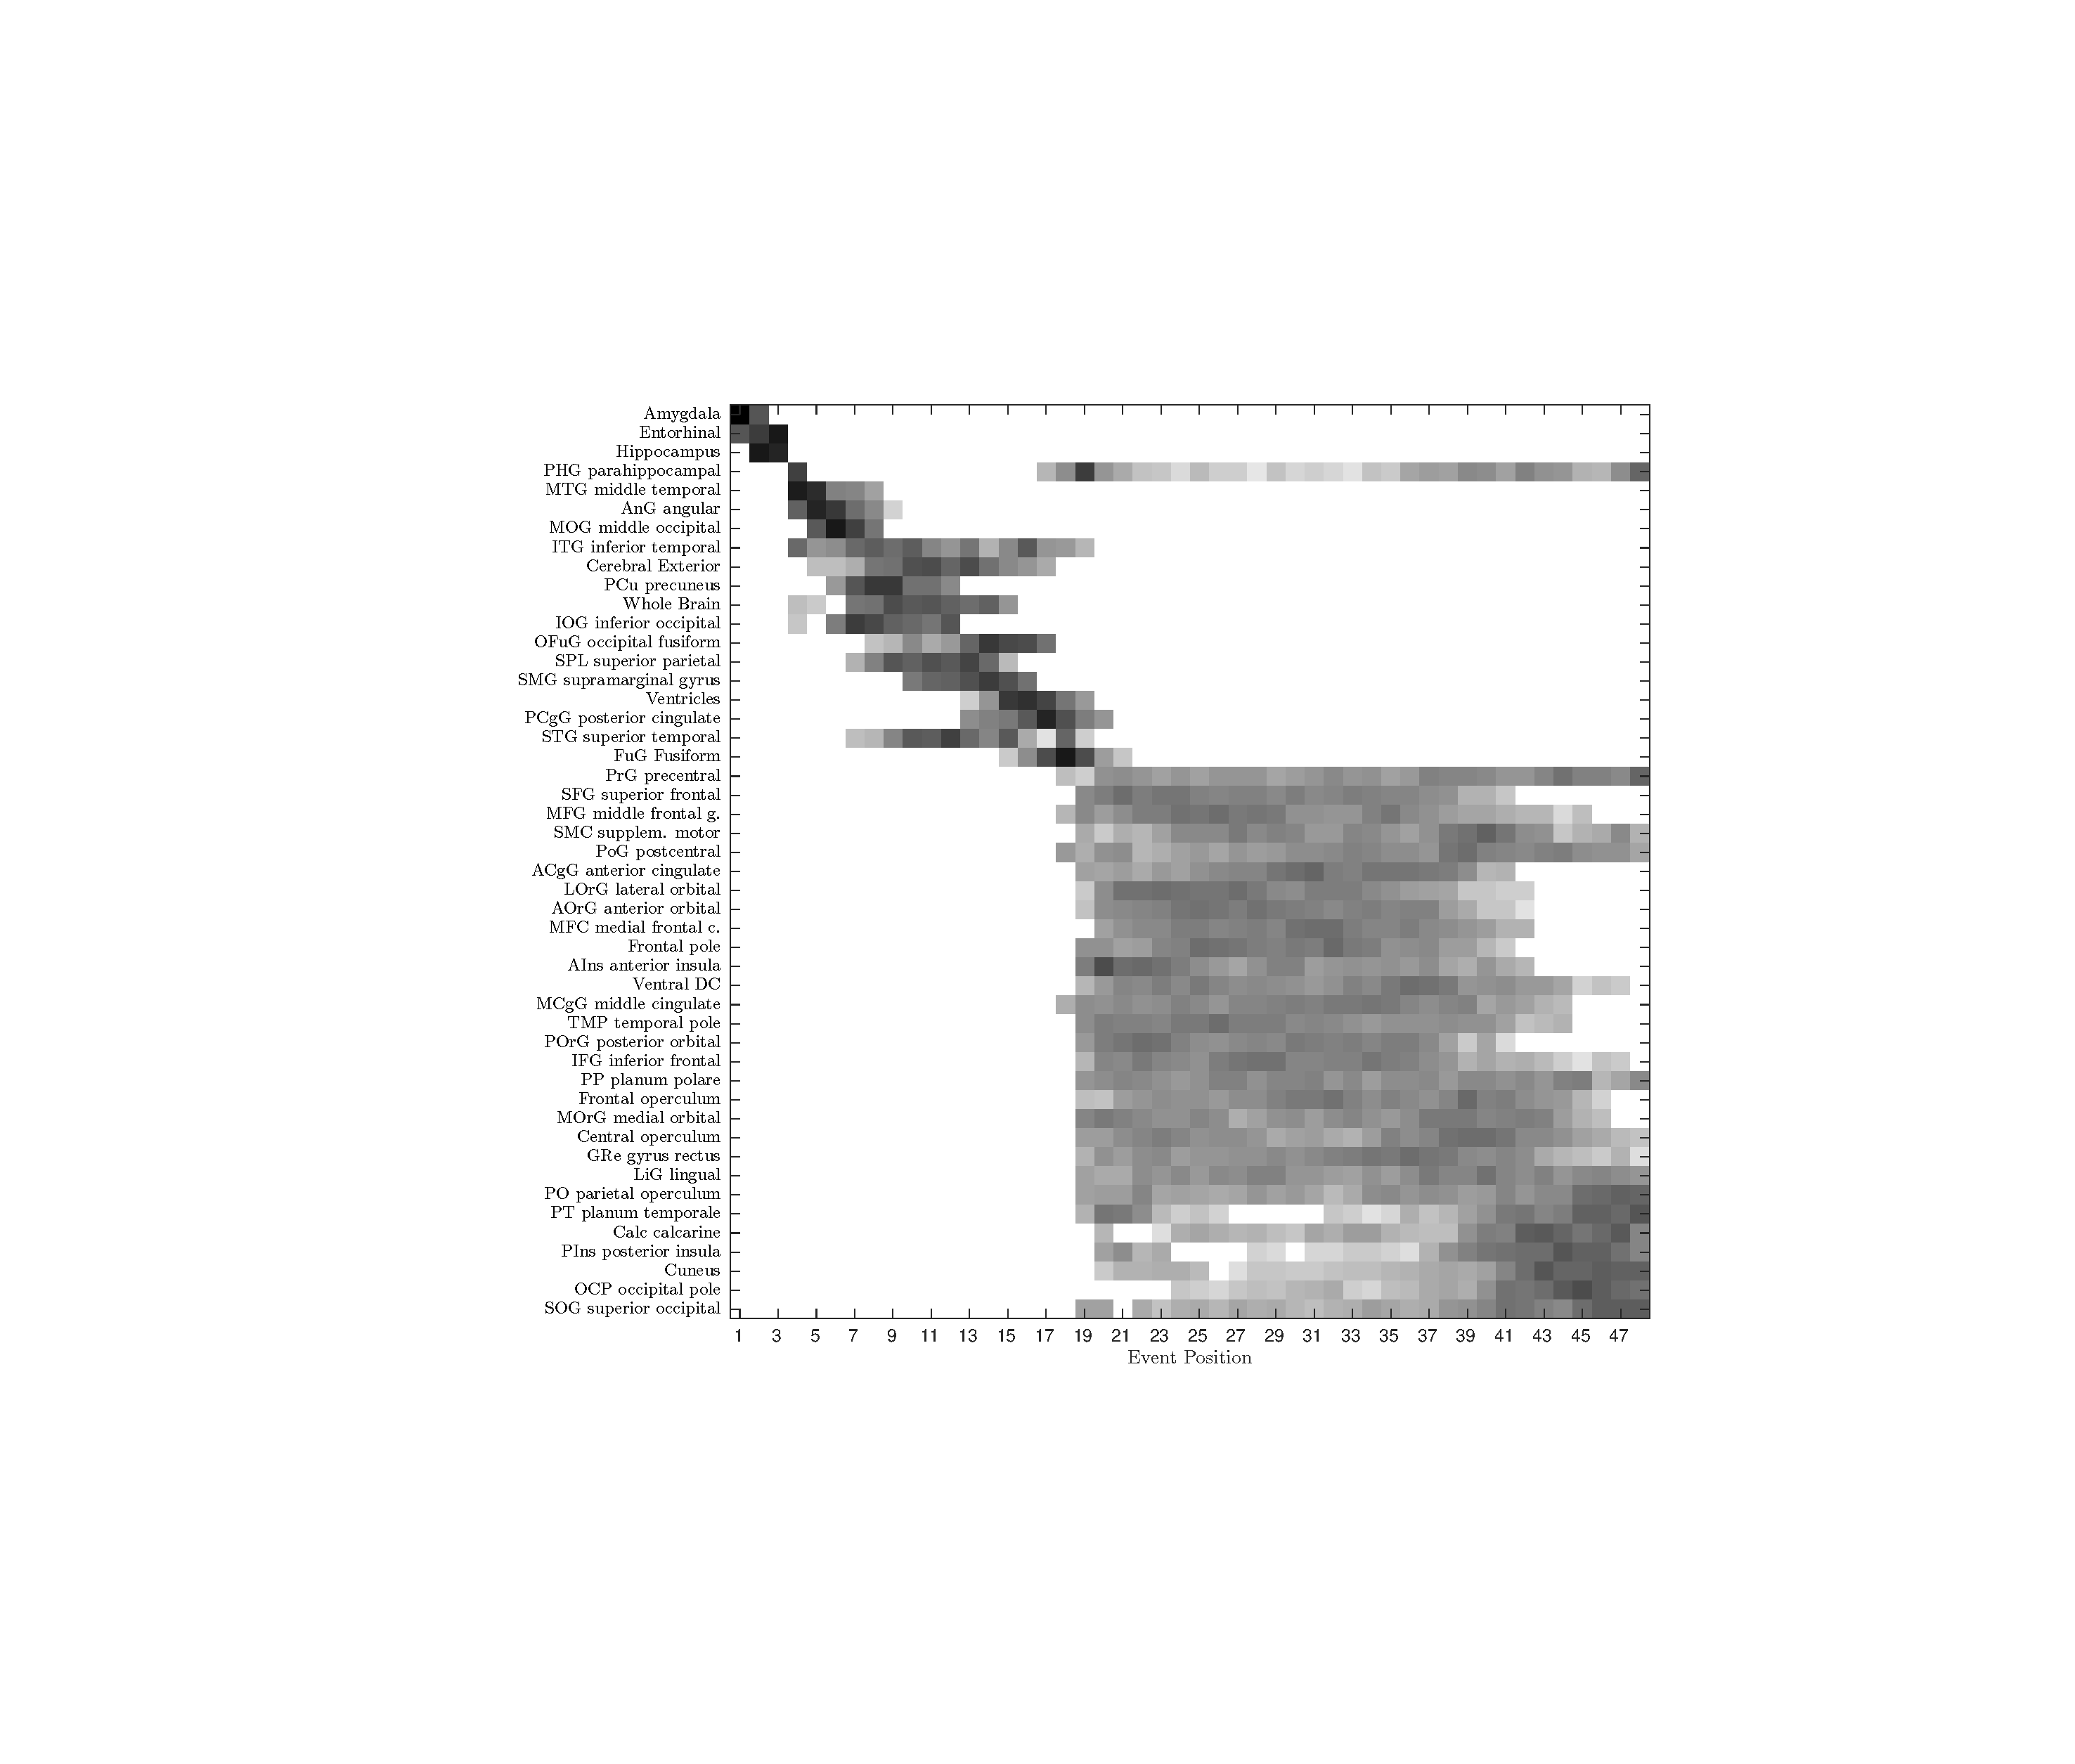
\includegraphics[scale=0.4]{../code/toyEBMs/figures/small5/posVarianceMatrix.pdf}};
  
  \draw (ordering.east) -| (1.5,0.3) -- (2.5,0.3);
  \draw (samples.east) -| (5.7,3);
  
  \draw (4,2.7) |- (7,3) -- (7,2.7);
  \draw (2.7,2) -| (2.5,-1.2) -- (2.7,-1.2);
  
\end{tikzpicture}
\caption[Event-based model - MCMC sampling diagram]{MCMC sampling and positional variance computation. MCMC sampling finds a series of $T$ samples, which are then used to derive the \emph{characteristic ordering}, where events are ordered according to their average position in the MCMC samples. Entries $M(i,j)$ in the positional variance matrix stores the relative number of times each event appeared in each position in the sequence. The events in the positional variance matrix are ordered according to the characteristic ordering.}
\end{figure}


\subsection{Event Sequence Estimation}
\label{sec:model_est}

Applying Bayes' theorem  we can get the posterior on the sequence:

\begin{equation}
 p(S|X) = \frac{p(S)p(X|S)}{p(X)}
\end{equation}

As the marginal distribution $p(X)$ is analytically intractable, one can use a Markov-chain Monte Carlo (MCMC) algorithm to sample from the posterior $p(S|X)$. A detailed description on how the MCMC algorithm works is given is section \ref{sec:MCMC}. One assumes flat priors on the sequence $S$ as any sequence could be equally likely.

In the MCMC phase, at each iteration the sequence $S$ can be perturbed by swapping two randomly chosen events. This perturbation rule has been used by Fonteijn et al. \cite{fonteijn2012event}. However, another perturbation method used by Young et al. \cite{young2014data} randomly selects a source and target event and places the source event after the target event, sliding the other biomarkers accordingly. See figure \ref{fig:backgr_mcmc_perturb} for a representation of the two perturbation rules. The resulting sequence $S^{new}$ is accepted with probability $p = min(1, a)$ where $ a = p(X|S^{new})/p(X|S)$. Otherwise the old sequence is stored and the process is repeated. As MCMC depends on accurate initialisation, one also runs a greedy ascent algorithm in order to find the sequence with the highest likelihood. The greedy ascent is very similar to the MCMC phase, the only difference being that $a$ is set to 1 if $p(X|S^{new}) > p(X|S)$ and to zero otherwise. Depending on the number of biomarkers, the greedy ascent is run for a few thousand iterations and repeated 10 times, with different random permutations of integers $1,\dots,N$ as the starting position. The maximum likelihood sequence obtained from greedy ascent is then used to initialise MCMC sampling, which usually runs for at least 100,000 iterations, again depending on problem size.

The resulting MCMC-sampled sequences are usually plotted in a positional variance matrix $M$, which is a compact way to represent uncertainty in the event ordering. Each element $M(i,j)$ represents the proportion of times event $E_{s(i)}$ appeared on position $j$ in the sampled sequences, given some \emph{master sequence} $S$. $S$ is usually set to be the maximum likelihood sequence or the \emph{characteristic ordering}, which is given by the average position of the events in the MCMC samples \cite{fonteijn2012event}. The characteristic sequence is particularly useful in plotting positional variance matrices from cross-validation or bootstrapping.

\begin{figure}
\centering
\begin{subfigure}[b]{0.45\textwidth}
 \centering
 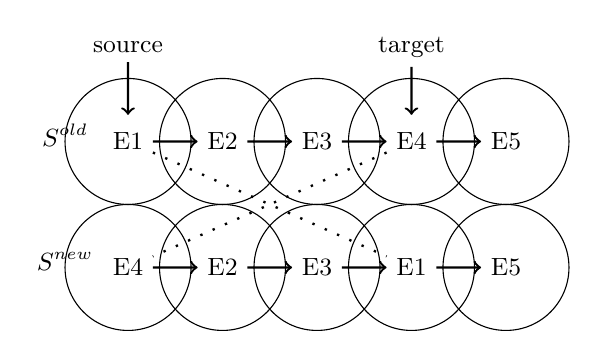
\begin{tikzpicture}[scale=0.8]
  \tikzstyle{every node}=[font=\small]


  \draw (-5,3) circle [radius=\nodeRad] node (E1) {E1};
  \draw (-3.5,3) circle [radius=\nodeRad] node (E2) {E2};  
  \draw (-2,3) circle [radius=\nodeRad] node (E3) {E3};
  \draw (-0.5,3) circle [radius=\nodeRad] node (E4) {E4};
  \draw (1,3) circle [radius=\nodeRad] node (E5) {E5};  
  \node (descold) at (-6,3.1) {$S^{old}$};
  \node (src) at (-5,4.5) {source};
  \node (trg) at (-0.5,4.5) {target};
  
  \draw[->,line width=0.3mm] (E1) -- (E2);
  \draw[->,line width=0.3mm] (E2) -- (E3);
  \draw[->,line width=0.3mm] (E3) -- (E4);
  \draw[->,line width=0.3mm] (E4) -- (E5);
  \draw[->,line width=0.3mm,shorten >=3pt] (src) -- (E1);
  \draw[->,line width=0.3mm,shorten >=3pt] (trg) -- (E4);  
  
  \draw (-5,1) circle [radius=\nodeRad] node (E4b) {E4};
  \draw (-3.5,1) circle [radius=\nodeRad] node (E2b) {E2};  
  \draw (-2,1) circle [radius=\nodeRad] node (E3b) {E3};
  \draw (-0.5,1) circle [radius=\nodeRad] node (E1b) {E1};
  \draw (1,1) circle [radius=\nodeRad] node (E5b) {E5};
  \node (descnew) at (-6,1.1) {$S^{new}$};
  
  \draw[->,line width=0.3mm] (E4b) -- (E2b);
  \draw[->,line width=0.3mm] (E2b) -- (E3b);
  \draw[->,line width=0.3mm] (E3b) -- (E1b);
  \draw[->,line width=0.3mm] (E1b) -- (E5b);
  
  \draw[loosely dotted, line width=0.3mm] (E1) -- (E1b);
  \draw[loosely dotted, line width=0.3mm] (E4) -- (E4b);  
 
  
\end{tikzpicture}
\caption{Fonteijn et al. \cite{fonteijn2012event}}
\end{subfigure}
%   ~
\begin{subfigure}[b]{0.45\textwidth}
 \centering
 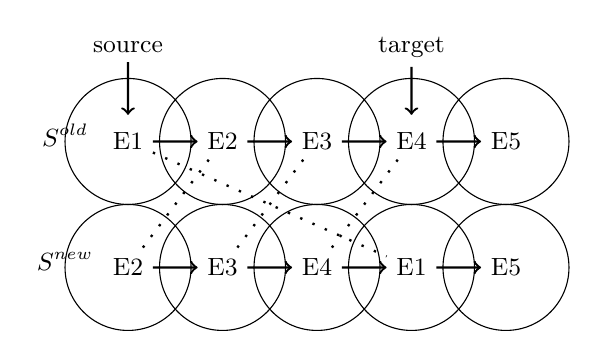
\begin{tikzpicture}[scale=0.8]
  \tikzstyle{every node}=[font=\small]


  \draw (-5,3) circle [radius=\nodeRad] node (E1) {E1};
  \draw (-3.5,3) circle [radius=\nodeRad] node (E2) {E2};  
  \draw (-2,3) circle [radius=\nodeRad] node (E3) {E3};
  \draw (-0.5,3) circle [radius=\nodeRad] node (E4) {E4};
  \draw (1,3) circle [radius=\nodeRad] node (E5) {E5};  
  \node (descold) at (-6,3.1) {$S^{old}$};
  \node (src) at (-5,4.5) {source};
  \node (trg) at (-0.5,4.5) {target};
  
  \draw[->,line width=0.3mm] (E1) -- (E2);
  \draw[->,line width=0.3mm] (E2) -- (E3);
  \draw[->,line width=0.3mm] (E3) -- (E4);
  \draw[->,line width=0.3mm] (E4) -- (E5);
  \draw[->,line width=0.3mm,shorten >=3pt] (src) -- (E1);
  \draw[->,line width=0.3mm,shorten >=3pt] (trg) -- (E4);  
  
  \draw (-5,1) circle [radius=\nodeRad] node (E2b) {E2};
  \draw (-3.5,1) circle [radius=\nodeRad] node (E3b) {E3};  
  \draw (-2,1) circle [radius=\nodeRad] node (E4b) {E4};
  \draw (-0.5,1) circle [radius=\nodeRad] node (E1b) {E1};
  \draw (1,1) circle [radius=\nodeRad] node (E5b) {E5};
  \node (descnew) at (-6,1.1) {$S^{new}$};
  
  \draw[->,line width=0.3mm] (E2b) -- (E3b);
  \draw[->,line width=0.3mm] (E3b) -- (E4b);
  \draw[->,line width=0.3mm] (E4b) -- (E1b);
  \draw[->,line width=0.3mm] (E1b) -- (E5b);
  
  \draw[loosely dotted, line width=0.3mm] (E1) -- (E1b);
  \draw[loosely dotted, line width=0.3mm] (E2) -- (E2b);
  \draw[loosely dotted, line width=0.3mm] (E3) -- (E3b);
  \draw[loosely dotted, line width=0.3mm] (E4) -- (E4b);  
 
  
\end{tikzpicture}
\caption{Young et al. \cite{young2014data}}
\end{subfigure}

\caption[MCMC perturbation rules]{MCMC perturbation rules used by (a) Fonteijn et al. \cite{fonteijn2012event} and (b) Young et al. \cite{young2014data}. Both methods assume randomly selected source and target events. The method by Fonteijn et al. only swaps the source event (E1) with the target event (E4). On the other hand, the perturbation used by Young et al. moves a source event after a target event and slides the other biomarkers accordingly.}
\label{fig:backgr_mcmc_perturb}
\end{figure}

\subsection{MCMC sampling - Metropolis Hastings}
\label{sec:MCMC}

%TODO: picture with proposal and sampling distribution

In order to sample the event ordering, one can use the Metropolis Hastings algorithm, which is a Markov chain Monte Carlo sampling  method. The original Metropolis algorithm was proposed by Metropolis et al. in 1953 \cite{metropolis1953equation}. W. K. Hastings extended it to a more general case in 1970 \cite{hastings1970monte}. 

Suppose we have a function $f(x)$ which is proportional to a probability distribution $p(x)$, which we need to take samples from. It is often the case in practice that the normalisation factor is not known because it is extremely difficult to compute it. The Metropolis Hastings algorithm works by producing a sequence of samples $X_0,X_1,\dots,X_n$ where each sample $X_{t+1}$ is generated from $X_t$ using a proposal distribution $Q(X_{t+1}|X_t)$. At each iteration, a candidate sample $X_{cand}$ is generated from the proposal distribution $Q(X_{t+1}|X_t)$. A probability ratio $a$ is calculated as follows:

\begin{equation}
 a = \frac{f(X_{cand})}{f(X_{t})} \frac{Q(X_t|X_{cand})}{Q(X_{cand}|X_t)}
\end{equation}
Finally, the sample $X_{cand}$ is accepted with probability $\min(1, a)$. Note that in most cases the \emph{proposal distribution} is symmetric, i.e. $Q(X_t|X_{cand}) = Q(X_{cand}|X_t)$, in which case the ratio $a$ becomes:

$$a = \frac{f(X_{cand})}{f(X_{t})}$$

\begin{myalgo}[Metropolis-Hastings algorithm]
 \begin{enumerate}[label*=\arabic*.]
  \item Choose a starting point $X_1$
  \item for $t=2$ to $T$
  \begin{enumerate}[label*=\arabic*.]
    \item Draw a candidate sample $X^{cand}$ from the proposal distribution $Q(X|X^t)$
    \item Compute the acceptance ratio $a$ as follows:
       $$a = \frac{f(X_{cand})}{f(X_{t})} \frac{Q(X_t|X_{cand})}{Q(X_{cand}|X_t)}$$
    \item Draw a random number $r$ from the unit interval $[0,1]$
    \item Accept the candidate sample $X^{cand}$ only if $a \ge r$. That is:
       $$ X^{t+1} = \begin{cases} \hfill X^{cand} &\mbox{if } a \ge r \\ 
					      X^t & \mbox{ otherwise }\end{cases}$$
    
  \end{enumerate}
  
 \end{enumerate}

\end{myalgo}


\subsection{Mixture Models For Data Likelihood}
\label{sec:mix_models}

In equation \ref{eq:ebm1} we need to model the distributions $p\left(x_{i,j} | E_{i} \right)$ and $p\left(x_{i,j} | \neg E_{i}\right)$ using the measurements in $X$. However, the fact that a subject is a control or patient does not give any information whether event $E_{i}$ has occurred. Therefore, it is necessary to use a mixture model, whose components will correspond to $p\left(x_{i,j} | E_{i} \right)$ and $p\left(x_{i,j} | \neg E_{i}\right)$ respectively. The particular choice of the model depends on the data that is being modelled. Fonteijn et al. \cite{fonteijn2012event} used a Gaussian distribution for $p\left(x_{i,j} | \neg E_{i}\right)$ and a uniform distribution for $p\left(x_{i,j} | E_{i} \right)$. On the other hand, Young et al. \cite{young2014data} used two Gaussian distributions for both distributions and applied some constraints on their mean and variance. The models are fit using numerical optimisation or Expectation-Maximisation (EM).

\subsection{Patient Staging and Diagnosis Prediction}
\label{sec:staging}

After the maximum likelihood sequence has been found using the greedy ascent method described in section \ref{sec:model_est}, each subject can be assigned a stage $k$ as follows:

\begin{equation}
\label{eq:staging}
 k = \argmax_k p(k) p(X_j | S, k) = p(k) \prod_{i=1}^k p\left(x_{s(i),j} | E_{s(i)} \right) \prod_{i=k+1}^N p\left(x_{s(i),j} | \neg E_{s(i)}\right) 
\end{equation}
 

As before, the prior $p(k)$ is assumed to be uniform. It should be noted that stages range from zero to $N$, the number of events. If a subject is at stage $k$ it means that all events up to and including $k$ have occurred while the events after $k$ have not occurred. 

One can use patient stages to classify subjects into controls and AD, or any other available subgroups, using a simple method by Young et al. \cite{young2014data}. Given a threshold stage $t$, one can predict all subjects having a stage less than or equal to $t$ to be controls and all subjects with stages greater than $t$ to be patients. The optimal threshold is the one which maximises the balanced accuracy, defined as follows:

\begin{equation}
 Accuracy = \frac{TP + TN}{TP + FP + FN + TN}
\end{equation}
where $TP$, $FP$, $FN$, $TN$ represent the number of true positive, false positive, false negative and true negative subjects respectively. After the optimal threshold is found, one can also compute the sensitivity and specificity defined as follows:

\begin{equation}
 Sensitivity = \frac{TP}{TP + FN}
\end{equation}

\begin{equation}
 Specificity = \frac{TN}{TN + FP}
\end{equation}



\subsection{Advantages and Limitations}

% Advantages
The event-based model by Fonteijn et al. \cite{fonteijn2012event} has several advantages. It is a data-driven progression model which does not use a-priori defined clinical stages, which can often be biased and limit the temporal resolution of the model. Moreover, it does not require longitudinal data, which makes it very useful for analysing rare types of dementia for which comprehensive longitudinal datasets do not exist. The Bayesian framework in which it is formulated also allows it to estimate uncertainty in the abnormality sequence. The model can also easily combine data from different modalities.  

% Limitations
The current model has several limitations. The trajectory parameters are modelled as step functions, which is a strong assumption given the continuous nature of almost every MRI and CSF biomarker commonly used in the field. Secondly, in the fitting process the parameters and sequence are assumed independent and therefore fitted separately. Third, the model assumes all biomarker measurements are independent with each other and also across different visits of the same subject.  Finally, the model also assumes that all subjects follow the same progression sequence, which is not the case in heterogeneous datasets such as ADNI.


\section{Differential Equation Model}
\label{sec:dem}

The differential equation model (DEM) \cite{ashford2001modeling,yang2011quantifying,sabuncu2011dynamics,villemagne2013amyloid} constructs the biomarker trajectories from the change in biomarker values between different visits. In many datasets such as ADNI, the biomarker scores $s$ are observed for each subject over a few visits. By determining how these scores change ($\Delta s$) over time ($t$) during a specified time interval $\Delta t$, the temporal rate of progression ($\Delta s/\Delta t$) can be modelled as a function of the mean biomarker value $f(s)$ \cite{ashford2001modeling}:

\begin{equation}
\label{eq:dem_1}
 \frac{\Delta s}{\Delta t} \approx f(s)
\end{equation}

The model given by $f(s)$ can be for example linear, polynomial or non-parametric models such as Gaussian Processes (GP). We then perform a line integral along $f(s)$ to recover $s(t)$. More explicitly, if we take the limit as $\Delta \xrightarrow{} 0$ from Eq. \ref{eq:dem_1}, we get that:

\begin{equation}
\label{eq:dem2}
lim_{\Delta t \xrightarrow{}  0} \frac{\Delta s}{\Delta t} = \frac{\delta s}{\delta t} = f(s)
\end{equation}

Solving this numerically is done using the Euler method. We set an initial $(t_0,s_0)$ and small increment step $\delta t$ and finding the next pair $(t_1, s_1)$ as follows:

\newcommand\numberthis{\addtocounter{equation}{1}\tag{\theequation}}

\begin{align*}
 t_1 &= t_0 + \delta t \\
 s_1 &= s_0 + f(s_0) \delta t \numberthis \label{eq:dem3}
\end{align*}

This is the repeated until the full curve defined by $(t_0, s_0), (t_0, s_0), \dots, (t_n, s_n)$ is reconstructed. The process is repeated independently for the other biomarkers. 

\subsection{Advantages and Limitations}

The differential equation model has several advantages. It is a fully data-driven method that does not require a-priori defined clinical categories. In contrast to the event-based model, it can estimate non-parametric biomarker trajectories which makes minimal assumptions on the shape of the biomarker trajectories, with the only real constraint being monotonicity. 

The model has several limitations. First of all, the biomarker trajectories are fit independently, which requires alignment on the temporal axis after they are recovered. Secondly, in this formulation the model does not allow to directly estimate uncertainty in the trajectory values along the y-axis. The only option for estimating uncertainty is by integrating posterior samples of the differential model and then aligning them all on the temporal axis. A third limitation is that the model is very sensitive to noise in the biomarker measurements. 


\section{The Disease Progression Score model}
\label{sec:dps}

The disease progression score (DPS) model was proposed by Jedynak et al. \cite{jedynak2012computational}. It is based on three main assumptions:
\begin{itemize}
 \item Subjects follow a common disease progression but they have a different age on onset and progression speed.
 \item Each biomarker trajectory is a monotonic curve that follows a sigmoidal shape
 \item The speed of progression of each subject is the same across the entire disease time-course.
\end{itemize}

The model estimates the optimal shape of the biomarker trajectories while estimating a disease progression score for each subject, which is the stage along the disease time course. The disease progression score $s_{ij}$ for subject $i$ at visit $j$ is defined as a linear transformation of age $t_{ij}$:

\begin{equation}
\label{eq:dps}
 s_{ij} = \alpha_i t_{ij} + \beta_i
\end{equation}
% sigmoidal functions
where $\alpha_i$ and $\beta_i$ represent the speed of progression and time shift (i.e. disease onset) of subject $i$. 

The DPS model assumes that biomarker measurements are independent and follow a sigmoidal trajectory $f(s)$ given the disease progression score $s$. The sigmoidal function for biomarker $k$ is parametrised as $\theta_k = [a_k,b_k,c_k,d_k]$ where:

\begin{equation}
 f(s;\theta_k) = \frac{a_k}{1+exp(-b_k(s-c_k))} + d_k
\end{equation}
where $d_k$ is the minimum value, $d_k+a_k$ is the maximum value, $a_kb_k/4$ is the maximum slope and $c_k$ is the inflexion point. Previous work has shown that sigmoidal curves provide a better fit for biomarker data compared to linear models \cite{sabuncu2011dynamics,caroli2010dynamics}. The value $y_{ijk}$ of biomarker $k$ from subject $i$ at visit $j$ is a normally distributed random variable:
\begin{equation}
 p(y_{ijk} | \alpha_i, \beta_i, \theta_k, \sigma_k) = N(y_{ijk} | f(\alpha_i t_{ij} + \beta_i; \theta_k), \sigma_k )
\end{equation}
We further define $I$ to be the set of all triplets $(i,j,k)$ for which measurements are available. Assuming independence across all measurements we get the following model likelihood:
\begin{equation}
 p(y | \alpha, \beta, \theta, \sigma) = \prod_{(i,j,k) \in I} p(y_{ijk} | \alpha_i, \beta_i, \theta_k, \sigma_k)
\end{equation}
where $y = [y_{ijk}]$ for $(i,j,k) \in I$. Vectors $\alpha = [\alpha_1, \dots, \alpha_S]$ and $\beta = [\beta_1, \dots, \beta_S]$, where $S$ is the number of subjects, denote the stacked parameters for the subject shifts. Vectors $\theta = [\theta_1, \dots, \theta_K]$ and $\sigma = [\sigma_1, \dots, \sigma_K]$, with $K$ being the number of biomarkers, represent the stacked parameters for the sigmoidal trajectories and measurement noise specific to each biomarker.

The parameters of the model are therefore $\Theta = [\alpha, \beta, \theta, \sigma]$ and the log-likelihood function associated with it is:
\begin{equation}
 l(\alpha, \beta, \theta, \sigma) = \sum_{(i,j,k) \in I} log \sigma_k + \frac{1}{2 \sigma_k ^2} \left( y_{ijk} - f(\alpha_i t_{ij})\right)
\end{equation}

\subsection{Model fitting}

Model fitting is done by alternating between optimising the sigmoidal parameters $\sigma$ and the subject specific parameters $\alpha, \beta$ using the method of least squares. Figure \ref{fig:algo_dps} show the fitting procedure. In line \ref{alg:init}, we initialise $\alpha_i = 1$, $\beta_i = 0$ for every $i$. On lines \ref{alg:theta} and \ref{alg:sigma} the optimal parameters for every biomarker trajectory are computed. On line \ref{alg:alpha} the subject specific shifts and progression speeds are found. Sometimes unfeasible parameters can be retrieved, so on line \ref{alg:identif} the parameters are mapped into the feasible space. In order to make the model identifiable, parameters $\alpha_i$ and $\beta_i$ are rescaled for every subject on line \ref{alg:rescale} so that the disease progression scores of healthy controls have a mean $\mu_N$ of 0 and a standard deviation $\sigma_N$ of 1.

\begin{algorithm}
%  \KwData{this text}
%  \KwResult{how to write algorithm with \LaTeX2e }
 Initialise $\alpha^{(0)}$, $\beta^{(0)}$\;\label{alg:init}
 \For{$l=1$ to $L$}{
    \For{$k=1$ to $K$}{
      $\theta_k^{(1)} = \argmin_{\theta_k} \sum_{(i,j) \in I_k} (y_{ijk} - f(\alpha_i^{(0)} t_{ij} + \beta_i^{(0)} | \theta_k))^2$\label{alg:theta}\\
      $\sigma_k^{(1)^2} = \frac{1}{|I_k-2I-4|} \sum_{(i,j) \in I_k} (y_{ijk} - f(\alpha_i^{(0)} t_{ij} + \beta_i^{(0)} | \theta_k))^2$\label{alg:sigma}
    }
    \For{$i=1$ to $I$}{
      $\alpha_i^{(1)}, \beta_i^{(1)} = \argmin_{\alpha_i, \beta_i}  \sum_{(j,k) \in I_i} \frac{1}{\sigma_k^{(1)^2}}(y_{ijk} - f(\alpha_i t_{ij} + \beta_i | \theta_k^{(1)}))^2$\label{alg:alpha}
    }
    $\alpha^{(0)}=\alpha^{(1)}, \beta^{(0)}=\beta^{(1)}$\label{alg:update}
 }

  \For{$k=1$ to $K$}{
    \If{$b_k < 0$}{
      $a_k^{(1)} = -a_k^{(1)}, b_k^{(1)} = -b_k^{(1)}, d_k^{(1)} = d_k^{(1)}+a_k^{(1)}$\label{alg:identif}\\
    }
  }
  
  \For{$i=1$ to $I$}{
    $\alpha_i = \frac{\alpha_i}{\sigma_N}, \beta_i = \frac{\beta_i - \mu_N}{\sigma_N}$\label{alg:rescale}
  }
 \caption{The optimisation procedure for the disease progression score by \cite{jedynak2012computational}.}
 \label{fig:algo_dps}
\end{algorithm}


\subsection{Advantages and Limitations}

The model by Jedynak et al. \cite{jedynak2012computational} has several advantages. As opposed to the differential equation model, the model automatically aligns the biomarker trajectories on the temporal axis. Furthermore, compared to the event-based model by \cite{fonteijn2012event}, the biomarker trajectories are modelled as sigmoidal trajectories instead of step functions and each subject has an associated time shift and progression speed. 

The model has several limitations. The main limitation of this model is that the trajectories are assumed to be sigmoidal, which is not necessarily the case for many biomarkers in ADNI (e.g. MRI volumes or cortical thickness) that don't show any signs of plateauing. Furthermore, each subject is assumed to follow the same progression pattern, which is not true in many heterogeneous datasets such as ADNI.

\section{The Self-Modelling Regression model}
\label{sec:semor}

Self-modelling regression (SEMOR) is a method that fits several curves under the assumption of a common shape \cite{donohue2014estimating}. This approach has been used by Donohue et al. \cite{donohue2014estimating} to estimate non-parametric biomarker trajectories with linear subject-specific effects. We assume that $Y_{ij}$ is the measurement of biomarker $j$ in subject $i$, $g_j$ is a continuously differentiable monotone function, $\gamma_i \sim N(0, \sigma_{\gamma}^2)$ is the time shift for subject $i$. The model is defined as follows:
\begin{equation}
 \label{eq:semor1}
 Y_{ij}(t) = g_j(t +\gamma_i)+\alpha_{0ij} + \alpha_{1ij}t+\epsilon_{ij}(t)
\end{equation}
where $\alpha_{0ij}, \alpha_{1ij} \sim N(0, \Sigma_j)$ model a linear perturbation of the non-parametric trajectory $g_j$ for subject $i$ and biomarker $j$, $t$ is the time and $\epsilon_{ij}(t) \sim N(0, \sigma_j)$ is the measurement noise.  

\subsection{Parameter fitting}

Fitting the model is done by iteratively estimating each set of parameters $(g_j, \gamma_i, \alpha)$ until convergence of the Residual Sum of Squares (RSS). The algorithm makes use of the following residuals:
\begin{equation}
\begin{cases}
  R_{ij}^g(t) = Y_{ij}(t) - \alpha_{0ij} - \alpha_{1ij}t & \qquad E\left[ R_{ij}^g(t) | g_j, t, \gamma_i \right] = g_j(t+\gamma_i)\\
  R_{ij}^{\alpha}(t) = Y_{ij}(t) - g_j(t+\gamma_i) & \qquad E\left[ R_{ij}^{\alpha}(t) | \alpha_{0ij}, \alpha_{1ij}, t \right] = \alpha_{0ij} + \alpha_{1ij}t\\
  R_{ij}^{\gamma}(t) = t-g_j^{-1}(Y_{ij}(t)) & \qquad E\left[ R_{ij}^{\gamma}(t) | \gamma_i \right] \approx g_j^{-1}(g_j(t+\gamma_i))-t = \gamma_i\\  
\end{cases}  
\end{equation}

Using the above residuals, the model is fit by initialising $\gamma_i$ and iterating the following steps\cite{donohue2014estimating}:
\begin{enumerate}
 \item Given $\gamma_i$, estimate $g_j$ by setting $\alpha_{0ij} = \alpha_{1ij} = 0$ and iterating the following subroutine:
 \begin{enumerate}
  \item Estimate $g_j$ by a monotone curve fit on $R_{ij}^g(t)$
  \item Estimate $\alpha_{0ij}, \alpha_{1ij}$ using the linear mixed model of $R_{ij}^{\alpha}(t)$. Repeat steps a and b until convergence of each $RSS_j = \sum_{it} \left[ Y_{ij}(t)-g_j(t+\gamma_i)-\alpha_{0ij}-\alpha_{1ij}t \right]^2 $
 \end{enumerate}
 
 \item Given the estimated $g_j$, set $\alpha_{0ij} = \alpha_{1ij} = \epsilon_{ij}(t) = 0$ and estimate each $\gamma_i$ with the average of $R_{ij}$ over all $j$ and $t$. Steps 1 and 2 are repeated until convergence of the total $RSS = \sum_{ijt} \left[ Y_{ij}(t)-g_j(t+\gamma_i)-\alpha_{0ij}-\alpha_{1ij}t \right]^2 $

\end{enumerate}

\subsection{Advantages and limitations}

The model have many advantages. It robustly models the average trajectory using a non-parametric model, in contrast with previous approaches \cite{jedynak2012computational}. Moreover, it also models unique trajectories for each subject as linear deviations from the average trajectories using a mixed effects model. Each subject also has it's own temporal shift. 

One limitation of the model is that it does not model different progression speeds for each individual. Also, estimating all the subject-specific parameters $(\alpha_{0ij}, \alpha_{1ij}, \gamma_i)$ requires suitable priors and many longitudinal measurements, which might not be available in some datasets. Moreover, it also assumes that biomarker measurements are independent, which makes it unsuitable for modelling large sets of correlated biomarkers such as vertex-wise cortical thickness measures or voxel-wise amyloid burden. 

\section{The Manifold-based mixed effects model}
\label{sec:manifold}

The manifold-based mixed effects model was introduced by Schiratti et al. in 2015 \cite{schiratti2015mixed}. The model generalises a previous linear mixed effects model by \cite{datar2012mixed} to account for time shifts and describes it in a Riemannian manifold setting. Let us assume we observe $p$ individuals, each having $n_i$ observations obtained at times $t_{i,1} < \dots < t_{i,n_i}$, each having $y_i,1, \dots, y_{i,n_i}$ biomarker measurements. For a point $p_0 \in M$, $v_0 \in T_{p_0}M$ we define $\gamma_{p_0,t_0,v_0} = Exp_{t_0,p_0}(\alpha_iv_0)(.)$ as the geodesic which passes through point $p_0$ at time $t_0$ with velocity $v_0$. We also consider $t_{i,j}$ and $y_{i,j}$ as the age and measurement for one biomarker in subject $i$ at visit $j$. This gives us the following model:

\begin{equation}
\label{eq:manifold1}
 y_{i,j} = Exp_{t_0+\tau_i,p_0}(\alpha_iv_0)(t_i,j) + \epsilon_{i,j}
\end{equation}
where
\begin{equation}
\label{eq:manifold2}
\begin{cases}
  \alpha_i = exp(\nu_i)\\
  \nu_i \sim \bigotimes_{i=1}^p N(0, \sigma_{\nu}^2)\\  
  \tau_i \sim \bigotimes_{i=1}^p N(0, \sigma_{\tau}^2)\\  
  \epsilon_{i,j} \sim \bigotimes_{i,j} N(0, \sigma^2)\\  
\end{cases}
\end{equation}
The model assumes that each $\eta_i$ and $\tau_i$ are independent. The parameters of the model are $\theta = [p_0, t_0, v_0, \sigma_{\eta}, \sigma_{\tau}, \sigma]$. The model above can be re-written as:
\begin{align*}
  y_{i,j} &= \gamma_{p_0,t_0,v_0}(\alpha_iv_0(t_{i,j}-t_0-\tau_i))+\epsilon_{i,j}\\
          &= \gamma_i(t_{i,j})+\epsilon_{i,j} \numberthis \label{eq:manifold3}
\end{align*}
where $\gamma_i$ is the subject specific trajectory that is modelled as an affine reparametrisation of the average trajectory $\gamma_{p_0,t_0,v_0}$. The model described here is univariate. However, an extension of he model has been published by Schiratti et al. \cite{schiratti2015learning} which extends this framework to a multivariate analysis. 

\subsection{The straight lines model}

If we assign the canonical (i.e. Euclidean) metric to the manifold $M=\mathbb{R}$, we get the "straight lines" model:
\begin{equation}
 y_{i,j} = p_0 + \alpha_i v_0(t_{i,j}-t_0-\tau_i)+\epsilon_{i,j}
\end{equation}

\subsection{The logistic curve model}

Some biomarkers such as Mini-Mental State Examination or other cognitive tests are bounded in a specific interval that can be mapped to (0,1). In order to give the (0,1) interval a Riemannian manifold structure we need to equip it with a Riemannian metric. For all points $p_0 \in M$ we define $g_0$ to be the inner product $g_{p_0}(u,v) = uM(p_0)v$ where $M(p_0) = \frac{1}{p_0^2(1-p_0)^2)}$. This results in the geodesics of $M$ to be logistic curves of the form $t \rightarrow (1+a\ \text{exp}(-rt))^{-1} $ \cite{schiratti2015mixed}. Therefore, the model from Eq. \ref{eq:manifold1} writes:
\begin{equation}
 y_{i,j} = \left[ 1+\left(\frac{1}{p_0}-1\right)\text{exp}\left( -\frac{\alpha_iv_0}{p_0(1-p_0)}(t_{i,j}-t_0-\tau_i)\right) \right]^{-1}+\epsilon_{i,j}
\end{equation}

\subsection{Advantages and limitations}

The model has several strengths and weaknesses. The main strength lies in the flexible Riemannian manifold framework, that allows one to create different models depending on how the inner product is defined. Moreover, the model estimates subject specific trajectories $\gamma_i$, time shifts $\tau_i$ and progression speeds $\alpha_i$. However, one of the limitations of the model is that it assumes a parametric form of the biomarker trajectories (i.e. sigmoidal). 

\section{The voxelwise disease progression model}
\label{sec:bilgel_voxelwise}

A voxelwise disease progression model has been introduced in 2016 by Bilgel et al. \cite{bilgel2016multivariate}. This model allows the discovery of patterns of atrophy that are not confined to a given region of interest (ROI). Since the input data is represented by voxel-wise measurements such as amyloid burden, a spatial correlation function is used to model correlation between voxel values. The model is built on the framework of the disease progression score by Jedynak et al. \cite{jedynak2012computational}. 

Let us assume that $t_{ij}$ represent the age for subject $i$ at visit $j$. The progression score $s_{ij}$ for subject $i$ at visit $j$ is an affine transformation of age $t_{ij}$:

\begin{equation}
 \begin{cases}
 s_{ij} = \alpha_i t_{ij} + \beta_i = \textbf{q}_{ij}^T\textbf{u}_i\\
 \textbf{u}_i \sim N_2(\textbf{m}, V(\boldsymbol{\nu}))
\end{cases}
\end{equation}
where $\alpha_i$, $\beta_i$ are the progression speed and time shift of subject $i$, $\textbf{q}_{ij} = [t_{ij}, 1]^T$ and $\textbf{u}_{i} = [\alpha_i, \beta_i]^T$. The prior covariance matrix $V$ is modelled as a 2 $\times$ 2 positive definite matrix that has a Log-Cholesky parametrisation given by $\boldsymbol{\nu}$. More precisely, if we consider a matrix $U$ such that $V = UU^T$ and $U = \begin{bmatrix}
    U_{11} & U_{12} \\
    0 & U_{22}\\
\end{bmatrix}$, then $\boldsymbol{\nu} = [logU_{11}, logU_{12}, logU_{22}]$

Furthermore, let us denote by $\textbf{y}_{ij}$ the $K \times 1$ vector of biomarker measurements for subject $i$ at visit $j$. The longitudinal trajectories corresponding to these measurements are modelled as follows:

\begin{equation}
 \begin{cases}
  \textbf{y}_{ij} = \textbf{a}s_{ij}+\textbf{b}+\epsilon_{ij}\\
  \epsilon_{ij} \sim N_K(0,R(\boldsymbol{\lambda},\boldsymbol{\rho}))
 \end{cases}
\end{equation}
where $\textbf{a} = [a_1, \dots, a_K]^T$, $\textbf{b} = [b_1, \dots, b_K]^T$ are the coefficients of the linear model and $\epsilon_{ij}$ is the measurement noise that is independent and identically distributed across different subjects and visits. The matrix $R(\boldsymbol{\lambda},\boldsymbol{\rho})$ is the spatial covariance that is assumed to have the form $R = \Lambda C \Lambda$, where $\Lambda$ is a diagonal matrix with diagonal elements $\boldsymbol{\lambda}$ and $C$ is a correlation matrix that is parametrised by $\boldsymbol{\rho}$ \cite{bilgel2016multivariate}. This ensures that the matrix $R(\boldsymbol{\lambda},\boldsymbol{\rho})$ is positive definite. In order to model correlation among voxel measurements, the elements $C_{kk'}$ of matrix $C$ must be a function of the distance $d \equiv d(k,k')$ between voxels $k$ and $k'$. Several such options exist:
\begin{itemize}
 \item Exponential: $C_{kk'} = \text{exp}(-d/\rho)$
 \item Gaussian: $C_{kk'} = \text{exp}(-(d/\rho)^2)$
 \item Exponential: $C_{kk'} = \left(1+(d/\rho)^2\right)^{-1}$
 \item Spherical: $C_{kk'} = \left( 1 - \frac{3}{2}\frac{d}{\rho} + \frac{1}{2}\left(\frac{d}{\rho}\right)^{3} \right)$ if $d<\rho$
\end{itemize}
The model parameters are therefore $\boldsymbol{\theta} = [\textbf{m},\boldsymbol{\nu},\textbf{a},\textbf{b},\boldsymbol{\lambda},\boldsymbol{\rho}]$. The model is a mixed effects model where $\textbf{a}$, $\textbf{b}$ are the fixed effects and $\textbf{u}_i$ are the random effects. 

\subsection{Model fitting}

The model is fit using the Expectation-Maximisation (EM), described below. The complete data log-likelihood is:
\begin{align*}
 & l(\textbf{y}, \textbf{u}; \boldsymbol{\theta}) = \sum_i l(\textbf{y}_i, \textbf{u}_i; \boldsymbol{\theta}) =\\
 & -\frac{1}{2}\sum_{i,j}log|2\pi R|-\frac{1}{2}\sum_{i,j}\left(\textbf{y}_{ij}-Z_{ij}\textbf{u}_i-\textbf{b}\right)^T \\
 & -\frac{1}{2}\sum_{i} log|2\pi V|-\frac{1}{2}\sum_{i}(\textbf{u}_i-\textbf{m})^T V^{-1}(\textbf{u}_i-\textbf{m})
 \numberthis \label{eq:bilgel3}
\end{align*}

\subsubsection{E-step}

Let $(\textbf{y}, \textbf{u})$ be the complete data and $\boldsymbol{\theta}' = [\textbf{m}',\boldsymbol{\nu}',\textbf{a}',\textbf{b}',\boldsymbol{\lambda}',\boldsymbol{\rho}']$ be the parameters estimated at the previous EM iteration. Bilgel et al. \cite{bilgel2016multivariate} show that the E-step integral $Q(\boldsymbol{\theta}, \boldsymbol{\theta}')$ is proportional to $\sum_i \int \Phi(\tilde{\textbf{u}_i};\hat{\textbf{u}}'_i, \Sigma_i') l(\textbf{y}_i, \tilde{\textbf{u}}_i; \boldsymbol{\theta})d\tilde{\textbf{u}}_i$, where $\Phi$ is a multivariate normal probability density function with mean:

\begin{equation}
 \hat{\textbf{u}}'_i = \left( \sum_{j} Z'^T_{ij} R'^{-1} Z'_{ij} + V'^{-1}\right)^{-1}\left( \sum_{j} Z'^T_{ij} R'^{-1} (\textbf{y}_{ij}-\textbf{b}') + V'^{-1}\textbf{m}' \right)
\end{equation}
and covariance matrix $\Sigma'_{i}=\left( \sum_{j} Z'^T_{ij} R'^{-1} Z'_{ij} + V'^{-1}\right)^{-1}$. Evaluating the integral gives the following final form:

\begin{align*}
 & Q(\boldsymbol{\theta}, \boldsymbol{\theta}') = -\frac{1}{2} \sum_{ij}log|R| - \frac{1}{2}\sum_{ij}\left( \textbf{y}_{ij} - Z_{ij}\hat{\textbf{u}}'_i -\textbf{b}\right) - \frac{1}{2}\sum_{ij}Tr\left( Z^T_{ij} R^{-1} Z_{ij}\Sigma_i' \right) - \\
 & \frac{1}{2}\sum_{i}log|V| - \frac{1}{2}\sum_{i}\left( \hat{\textbf{u}}'_i - \textbf{m} \right)^T V^{-1} \left( \hat{\textbf{u}}'_i - \textbf{m} \right) - \frac{1}{2}\sum_i Tr\left( V^{-1} \Sigma_i'\right) \numberthis \label{eq:bilgel_e-step}
\end{align*}


\subsubsection{M-step}

At the M-step we need to find $\boldsymbol{\theta} = \argmax_{\boldsymbol{\theta}}Q(\boldsymbol{\theta}, \boldsymbol{\theta}')$. The full derivations are given in \cite{bilgel2016multivariate}, yielding the following updates:

\begin{equation}
\label{eq:bilgel_mstep1}
 \textbf{a} = \frac{\left( \sum_i \nu_i \right) \left( \sum_{ij} \textbf{y}_{ij}s'_{ij} \right) - \left( \sum_{ij} \textbf{y}_{ij} \right) \left( \sum_{ij}s'_{ij} \right)}{\left( \sum_i \nu_i \right) \left( \sum_{ij} \textbf{q}_{ij}^T \Sigma_i' \textbf{q}_{ij} + s_{ij}'^2 \right) - \left( \sum_{ij}s'_{ij} \right)^2}
\end{equation}

\begin{equation}
\label{eq:bilgel_mstep2}
 \textbf{b} = \frac{\left( \sum_{ij} \textbf{y}_{ij} \right) \left( \sum_{ij} \textbf{q}_{ij}^T \Sigma_i' \textbf{q}_{ij} + s_{ij}'^2 \right) - \left( \sum_{ij} \textbf{y}_{ij}s'_{ij} \right) \left( \sum_{ij} s'_{ij} \right)}{\left( \sum_i \nu_i \right) \left( \sum_{ij} \textbf{q}_{ij}^T \Sigma_i' \textbf{q}_{ij} + s_{ij}'^2 \right) - \left( \sum_{ij}s'_{ij} \right)^2}
\end{equation}

\begin{equation}
 \textbf{m} = \frac{1}{n}\sum_i \hat{\textbf{u}}'_i
\end{equation}

\begin{equation}
 \boldsymbol{\nu} = \argmax_{\boldsymbol{\nu}} Q(\boldsymbol{\theta}, \boldsymbol{\theta}')
\end{equation}

\begin{equation}
 \boldsymbol{\lambda}, \boldsymbol{\rho} = \argmax_{\boldsymbol{\lambda}, \boldsymbol{\rho}} Q(\boldsymbol{\theta}, \boldsymbol{\theta}')
\end{equation}

\subsection{Advantages and limitations}

The model by Bilgel et al. \cite{bilgel2016multivariate} has several advantages. First of all, it is specifically tailored for dealing with voxelwise measurements such as amyloid load by modelling the spatial correlations. Secondly, like the disease progression score by Jedynak et al. \cite{jedynak2012computational}, it estimates subject specific temporal shifts and progression speeds. 

The model has several limitations. First of all, the biomarker trajectories are assumed to be linear, which is a strong assumption especially for early many biomarkers such as amyloid, which start to plateau when subjects are in the MCI stages. Moreover, while it is necessary to incorporate a spatial correlation function due to the nature of the data, this has the effect of "blurring out" the image and is not suitable for some voxels that are close-by and undergo different trajectories. 

\section{The Network Diffusion Model}
\label{sec:diffusion_raj}

The network diffusion model was introduced by Raj et al. in 2012 \cite{raj2012network} and later extended in 2015 \cite{raj2015network}. The model is inspired by evidence that Alzheimer's disease atrophy spreading process occurs along vulnerable pathways in a prion-like manner rather than by spatial proximity \cite{villain2010sequential,englund1988white,kuczynski2010white}. The model works by simulating a diffusion process driven by concentration gradients along a connectivity graph that is obtained from tractography data of healthy controls. 

The diffusion process is modelled on a hypothetical brain network $G = \{V,E\}$ whose nodes $v_i \in V$ represent the gray matter structure of region $i$ and edges $(i,j)$ having weight $c_{ij}$ represent fibre connections between regions $i$ and $j$. Structures $v_i$ are obtained from parcellated regions-of-interest while the connection strength $c_{ij}$ is measured using tractography \cite{behrens2007probabilistic}. If we denote the disease factor in region $i$ as $x_i$, then the flow of the disease from a region $i$ to another region $j$ in a short time interval $\delta t$ is $\beta(x_i - x_j)c_{ij}\delta t$, where $\beta$ is a diffusivity constant controlling the diffussion speed. As $\delta t \to 0$, this results in the following first-order differential equation:
\begin{equation}
\label{eq:raj1}
 \frac{dx_j}{dt} = \beta c_{ij}(x_i - x_j)
\end{equation}
Now let us denote by $\textbf{x}(t) = \{x(v,t), v \in V \}$ the disease factor at time $t$ in every node of the network. Eq. \ref{eq:raj1} will then translate into the "network heat equation" \cite{kondor2002diffusion}:

\begin{equation}
\label{eq:raj2}
 \frac{d\textbf{x}(t)}{dt} = \beta H \textbf{x}(t)
\end{equation}
where $H$ is the Laplacian matrix of $G$ defined as:

\begin{equation}
\label{eq:raj3}
 H(i,j) = \begin{cases} 
 \sum_{j' \neq i} c_{ij'} & \mbox{for } i = j \\ 
 -c_{ij} & \mbox{otherwise} \\ 
\end{cases} 
\end{equation}
We model the cortical atrophy in region $k$ as the accumulation of the disease process:
\begin{equation}
\label{eq:raj4}
 \phi_k(t) = \int_0^t x_k(\tau)d\tau
\end{equation}
Extending this to the whole brain gives 
\begin{equation}
 \boldsymbol{\Phi(t)} = \int_0^t \textbf{x}(\tau)d\tau
\end{equation}
The solution to the above equation is given by:
\begin{equation}
 \textbf{x}(t) = \text{exp}(-\beta H t) \textbf{x}_0
\end{equation}
where $\textbf{x}_0$ is the initial disease concentration, where the term $\text{exp}(-\beta H t)$ acts as a smoothing operator. Performing eigenvalue decomposition on $H = U\Lambda U^{\dagger}$, where $U = [\textbf{u}_1,\dots,\textbf{u}_N]$ is the matrix of eigenmodes, allows to express $\textbf{x}(t)$ as:
\begin{equation}
 \textbf{x}(t) = U \text{exp}(-\Lambda \beta t) U^{\dagger} \textbf{x}_0 = \sum_{i=1}^N \left( \text{exp}(-\beta \lambda_i t) \textbf{u}_i^{\dagger} \textbf{x}_0 \right) \textbf{u}_i
\end{equation}
The time evolution of atrophy can then be described as:
\begin{equation} 
 \boldsymbol{\Phi}(t) = \int_0^t \sum_{i=1}^N \left( \text{exp}(-\beta \lambda_i t) \textbf{u}_i^{\dagger} \textbf{x}_0 \right) \textbf{u}_i\ dt = \sum_{i=1}^N \frac{1}{\beta \lambda_i} \left( 1-\text{exp}(-\beta \lambda_i t)\right) \textbf{u}_i^{\dagger} \textbf{x}_0 \textbf{u}_i 
\end{equation}
Raj et al. \cite{raj2012network} present evidence to suggest that the eigenmodes $\textbf{}_i$ with the highest corresponding eigenvalues $\lambda_i$ represent the areas that are normally affected by normal ageing, AD and behavioural variant frontotemporal dementia (bvFTD) respectively. They suggest that these areas are selectively vulnerable to these types of dementia, in line with previous findings in the literature \cite{seeley2009neurodegenerative,zhou2010divergent}. 

\subsection{Advantages and Limitations}

The diffusion model by Raj et al. \cite{raj2012network} has several advantages. In contrast with the models presented above, it is able to model the propagation of atrophy along white matter tracts, which can be used to test the prion hypothesis. Secondly, this approach allows one to test for hypothesis of network-based atrophy spread such as nodal stress, transneuronal spread, trophic failure, and shared vulnerability \cite{zhou2012predicting}.

The model has several limitations. The model assumes static networks, even though the network dynamically evolves during the time course of the disease. The model also assumes a parametric form of the biomarker trajectories, either exponential or sigmoidal.  

\section{Discriminative models}
\label{sec:backgr_svm}

Discriminative models such as Support Vector Machines (SVM) can also be used to model the progression of the disease. A Support Vector Machine is a non-probabilistic binary linear classifier that was originally developed by Vladimir N. Vapnik and Alexey Ya. Chervonenkis \cite{vapnik2006estimation}. They can perform non-linear classification by mapping the input data into higher-dimensional feature spaces using the \emph{kernel trick} and finding the hyperplane that optimally separates the data. They have been successfully used for differential diagnosis of different types of dementia using post-mortem confirmed subjects \cite{kloppel2008automatic}. Other uses of SVMs on medical images and other high-dimensional data have also been shown \cite{lao2004morphological,fan2005classification,mourao2005classifying,kawasaki2007multivariate}.

A different type of discriminative model is the random forest \cite{ho1995random,breiman2001random}. These work by building a multitude of decision trees on training data, using them to make predictions on the test data and performing majority voting on the predictions of individual trees to select the final labels. Random forests have been demonstrated in medical imaging for diagnosis classification \cite{gray2013random}, image quality transfer \cite{alexander2014image} or myocardium segmentation \cite{lempitsky2009random}. 

\subsection{Advantages and Limitations}

Discriminative models such as SVMs or random forests have several advantages. They work for a wide variety of problems, datasets and underlying models and are generally robust to high-dimensional data. Some of them such as random forests are also resistant to overfitting.

These discriminative models also have several fundamental limitations. First of all, they require labelled data, in the form of a-priori defined clinical categories or stages, which are usually coarse, inaccurate and biased. These limit the temporal resolution of the model. Moreover, it is also harder to interpret what these models learn from the data, which limits their use for understanding the disease process.

\begin{landscape}


\definecolor{orange0}{rgb}{1, 0, 0}
\definecolor{orange1}{rgb}{0.66, 0.33, 0}
\definecolor{orange2}{rgb}{0.33, 0.66, 0}
\definecolor{orange3}{rgb}{0, 0.7, 0}

\definecolor{green1}{rgb}{0, 0.6, 0}
\definecolor{red1}{rgb}{0.6, 0, 0}
\newcommand{\xmark}{\ding{55}}%

\newcommand{\myyes}{\textcolor{green1}{\Large{\checkmark}}}
\newcommand{\myno}{\textcolor{red1}{\Large{\xmark}}}
% \newcommand{}{×}

\begin{table}
\centering
\footnotesize
\renewcommand{\arraystretch}{1.5}% Spread rows out...
\begin{tabular}{>{\centering\arraybackslash}p{3.5 cm} | >{\centering\arraybackslash}p{2.5 cm} | >{\centering\arraybackslash}p{1.5 cm} | >{\centering\arraybackslash}p{1.5 cm} | >{\centering\arraybackslash}p{2.5 cm} | >{\centering\arraybackslash}p{2.5 cm} | >{\centering\arraybackslash}p{3 cm} | >{\centering\arraybackslash}p{3.5 cm}}
 Model & Trajectory shape & \multicolumn{2}{c|}{Subject Staging} & Handles Missing Data & Subject-specific trajectories & Models Biomarker Correlation & Main Limitation \\
 & & onset & speed & & & & \\
 \hline
 Discriminative Models & \textcolor{gray}{N/A} & \myno & \myno  & \myyes & \myno  & \myno & biased categories\\
  \hline
 Event-based Model & step-function & \myyes & \myno & \myno & \myno & \myno & no notion of time\\
  \hline
 Differential Equation Model & non-parametric & \myno * & \myno * & \myyes & \myno & \myno  & trajectories not aligned\\
  \hline
 Disease Progression Score & sigmoid & \myyes & \myyes & \myyes & \myno & \myno & sigmoidal trajectory assumption \\
  \hline
 Self-Modelling Regression & non-parametric & \myyes & \myyes & \myno & \myyes & \myno & requires large datasets \\
  \hline
 Manifold Model & linear, sigmoid & \myyes & \myyes & \myno & \myyes & \myno & sigmoidal trajectory assumption \\
  \hline
 Voxelwise Model & linear & \myyes & \myyes & \myyes & \myno & \myyes & linear trajectory assumption\\
  \hline
 Network diffusion Model & exponential, sigmoidal & \myno * & \myno *& \myno & \myno & \myyes & assumes static connectome\\

\end{tabular}
\caption{Comparison of features of various disease progression models. Models with * cannot be used for subject staging in their basic formulation, but extensions to the model can enable them to estimate subject-specific disease onset and progression speed.}
\label{tab:compDPMs}
\end{table}
\end{landscape}

\chapter{Project Data}
\label{chapter:methods_project_data}

For this project we used two main datasets: (1) the Alzheimer's Disease Neuroimaging Initiative (ADNI) and (2) the Dementia Research Center, UK (DRC) dataset. In sections \ref{sec:data_adni} and \ref{sec:data_drc} we present the subject demographics and how the data has been acquired and pre-processed. 

\section{ADNI dataset}
\label{sec:data_adni}

The ADNI dataset is a multisite, longitudinal study that assesses clinical, imaging, genetic and biospecimen biomarkers through the process of normal ageing to mild cognitive impairment (MCI) and dementia (AD) \cite{jack2008alzheimer}. Magnetic resonance imaging (MRI), (18F)-fluorodeoxyglucose positron emission tomography (FDG PET), urine serum and cerebrospinal fluid (CSF) data is acquired along with cognitive test information at multiple time points. At 55 participating sites in North America, the data was collected from 200 elderly cognitively normal, 400 MCI and 200 AD subjects. All subjects were scanned with 1.5T MRI at each time point and half of these were also scanned with FDG PET \cite{jack2008alzheimer}.  The main aims of the ADNI project was to make the data openly available to the scientific community, develop technical standards for imaging in longitudinal studies, find out optimal methods for image acquisition and analysis and validate imaging biomarkers by correlating them with cognitive tests. 

The ADNI dataset used for this project is the same one used by Young et al. in 2014 \cite{young2014data}. It was downloaded from LONI (www.loni.ucla.edu/ADNI/) on 5 February 2013 and included 285 subjects that had 1.5T MRI scans at baseline and 1 year, a CSF examination at baseline and cognitive tests at baseline which included the Mini-Mental State Examination (MMSE) \cite{mckhann1984clinical}, the Alzheimer's Disease Assessment Scale-Cognitive Subscale (ADAS-COG) \cite{rosen1984new} which omits item 13 (ADAS13) and the Rey Auditory Verbal Learning Test (RAVLT) \cite{rey1958examen}. FDG-PET and amyloid PET were not included in the dataset used by Young et al. \cite{young2014data}. CSF measures of amyloid beta, tau and total tau were performed centrally, and CSF tau and total tau were log transformed, to improve normality \cite{young2014data}. For the longitudinal analysis, imaging we used clinical and CSF data at 12- and 24-months follow-up periods. We also used the clinical diagnosis at all available timepoints up to 72 months. Demographics of the population analysed is included in table \ref{tab:adni_demographics}.

\rowcolors{1}{blue2}{white}
\begin{table}
\centering
\begin{tabular}{ c |C{1.7cm} | C{1.7cm} | C{2.5cm} | C{2.5cm} | C{1.7cm}} 
& \textbf{Number of Subjects} & \textbf{Gender} \hspace{1cm} M/F & \textbf{Age} \hspace{1cm} (years, mean $\pm$ SD) & \textbf{Education} (years, mean $\pm$ SD) & \textbf{APOE} \hspace{1cm} +/-\\
\textbf{Controls} & 92 & 48/44 (52\%) & 75 $\pm$ 5 & 15.6 $\pm$ 2.9 & 22/70 (24\%)\\ 
\textbf{MCI} & 129 & 82/47 (64\%) & 73 $\pm$ 7 & 15.9 $\pm$ 3 & 72/57 (56\%)\\ 
\textbf{AD} & 64 & 34/30 (53\%) & 75 $\pm$ 8 & 15 $\pm$ 3 & 45/19 (70\%)\\ 
\end{tabular}
\caption[Baseline population demographics for ADNI data]{Baseline population demographics for the ADNI cohort.}
\label{tab:adni_demographics}
\end{table}

\subsection{Image preprocessing}

The MRI acquisition protocols have already been detailed by Jack et al. in 2008 \cite{jack2008alzheimer}. In the dataset used for this project, cross-sectional brain regions of interest (ROIs) such as the hippocampus, entorhinal cortex, middle temporal gyrus, fusiform gyrus, ventricles and the whole brain, as well as total intracranial volume (TIV) were calculated at baseline and followup by Young et al.  \cite{young2014data} using Freesufer 4.3, a freely available brain imaging software (\url{http://www.freesurfer.net/}). All regional volumes were normalised by the total intracranial volume of each subject. The Boundary Shift Integral (BSI) \cite{freeborough1997boundary} was used to measure volume change between 0 and 12 months. The KN-BSI method by Leung et al. \cite{leung2010robust} was used to measure change in brain volume while the MAPS-HBSI method \cite{leung2010automated} was used to measure the hippocampal volume change. 

\section{DRC dataset}
\label{sec:data_drc}

The Dementia Research Center, UK provided us with a dataset of imaging data and cognitive test scores which contains healthy subjects along with subjects diagnosed with Alzheimer's disease (AD) and Posterior Cortical Atrophy (PCA). A total of 89 controls, 70 PCA and 65 AD subjects have been scanned with 1.5T/3T MRI at baseline. Some of them had follow-up scans for up to ten different timepoints. A total of 510 MRI scans have been acquired from these subjects at different timepoints. Demographic information about the DRC cohort is given in table \ref{tab:drc_demographics}.

\rowcolors{1}{blue2}{white}
\begin{table}
\centering
\begin{tabular}{ c |C{1.7cm} | C{1.7cm} | C{2.5cm} | C{2.5cm} | C{2.5cm}} 
& \textbf{Number of Subjects} & \textbf{Gender} \hspace{1cm} M/F & \textbf{Age at baseline} \hspace{1cm} (years, mean $\pm$ SD) & \textbf{Years from onset} (years, mean $\pm$ SD) & \textbf{Number of scans} (mean $\pm$ SD)\\
\textbf{Controls} & 89 & 33/56 & 60.5 $\pm$ 11 & - & 2.2 $\pm$ 1.3\\ 
\textbf{PCA} & 70 & 27/43 & 63.0 $\pm$ 7 & 4.4 $\pm$ 2.8 & 2.4 $\pm$ 1.4\\ 
\textbf{AD} & 65 & 34/31 & 66.3 $\pm$ 8 & 4.8 $\pm$ 2.6 & 2.1 $\pm$ 1.3\\ 
\end{tabular}
\caption[Baseline population demographics for DRC data]{Baseline population demographics for the DRC cohort.}
\label{tab:drc_demographics}
\end{table}


In order to perform tissue segmentation and parcellation, we used the Geodesic Information Flows (GIF) algorithm by Cardoso et al. \cite{cardoso2015geodesic} which is available for download at \url{http://cmictig.cs.ucl.ac.uk/niftyweb/}. The atlas that has been used for segmentation is the Neuromorphometrics atlas, which produced 146 different brain ROIs across the left and right hemisphere. The brain volumes have been corrected for total intracranial volume (TIV), age and gender using a linear regression approach. Left and right brain regions were averaged into one region. 
